Damit der Akku fachgerecht geladen wird, braucht es eine Ladeelektronik, welche den Lipo-Akku nach dem CCCV-Verfahren lädt. Es gab zwei Möglichkeiten wie man dies hätte aufbauen können. Die eine Möglichkeit ist ein teures IC gewesen, welches auf dem Markt verfügbar wäre, die andere Möglichkeit ist eine günstige Buck-Converter Schaltung, mit welchem man auch nach dem oberen Verfahren laden kann. Ein solcher Buck-Converter kommt nun in diesem Produkt zum Einsatz

\begin{figure} [H]
	\centering
	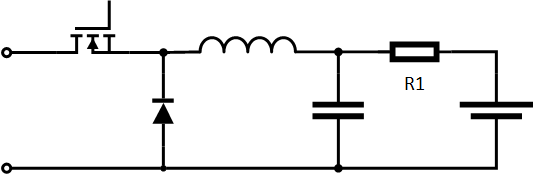
\includegraphics[width=0.6\linewidth]{images/Buck_Converter}
	\caption{Buck-Converter}
	\label{fig:Buck_Converter}
\end{figure}

Wie man in der vereinfachten Abbildung \ref{fig:Buck_Converter} des Buck-Converter sieht, ist dieser einfach und schnell aufgebaut. Der Widerstand R1 ist ein Shunt-Widerstand, an welchem der Strom gemessen wird. Anhand dieses Stromes wird der PWM, welcher über einen High-Side Treiber am Mosfet anliegt, durch den Mikrocontroller geregelt. Die Taktfrequenz des Clocks liegt bei 31.3kHz und wurde mit der Formel \eqref{eqn:Taktfrequenz} aus dem Datenblatt des Atmega berechnet.

\begin{equation}
f_{ PWM }=\frac { { f }_{ uC } }{ N*256 } 
\label{eqn:Taktfrequenz}
\end{equation}

Mit dieser Taktfrequenz kann man nun die grösse der Spule definieren. Dies wird mit folgender Formel \eqref{eqn:Spule} berechnet.

\begin{equation}
L=\frac { RF*\left( { V }_{ IN }-{ V }_{ OUT } \right) *\frac { { V }_{ OUT } }{ { V }_{ IN } }  }{ { f }_{ s }*{ I }_{ OUT } }  
\label{eqn:Spule}
\end{equation}

Berechnet wurde eine Spule von rund 120uH. Eingesetzt wurde eine Coilcraft-Spule mit dem Wert von 100uH. Da die Batterie wie ein grosser geladener Kondensator wirkt, sind keine all zu grossen Ripple am Ausgang des Buck-Converter zu erwarten.

\subsection*{Selbsterhaltung}
Wenn das Board voll geladen ist oder die fahrt für mehr als 20min unterbrochen wird, sollte es sich selbstständig herunterfahren und möglichst keinen Strom brauchen. Dafür wurde eine Selbsterhaltungsschaltung entwickelt (Abbildung \ref{fig:Selbsterhaltung}). Sobald beim Mikrocontroller einer von beiden Zustände eintrifft, wird der N-Kanal Mosfet ausgeschaltet. Somit wird die Speisung auf dem gesamten Print unterbrochen. Dadurch wird die Batterie bei einer längeren Lagerung vor dem zerstören geschützt.

\begin{figure} [H]
	\centering
	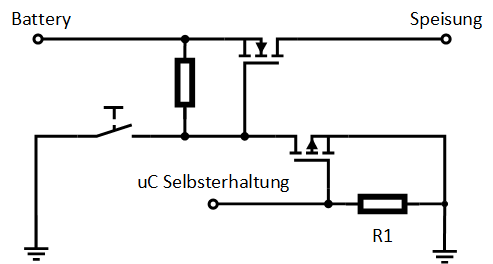
\includegraphics[width=0.6\linewidth]{images/Selbsterhaltung}
	\caption{Selbsterhaltung}
	\label{fig:Selbsterhaltung}
\end{figure}




